\documentclass[12pt]{article}
\usepackage[utf8]{inputenc}
\usepackage{amsmath}
\usepackage{graphicx}
\usepackage{float}
\usepackage[margin=1in]{geometry}
\usepackage{lineno}
\setlength{\parskip}{1em}
\renewcommand{\baselinestretch}{1.5}
\newcommand\dbyd[2]{\frac{\mathrm d{#1}}{\mathrm d{#2}}}
\newcommand\dsided[2]{{\mathrm d{#1}}/{\mathrm d{#2}}}
\newcommand{\R}{\mathcal{R}}
\title{Some plots I made to fix/answer some of the problems in my draft}
\author{Roger Zhang}
\date{June 24th 2018}
\usepackage{color}
\newcommand{\david}[1]{\textcolor{blue}{$\langle${\slshape{\bfseries David:} #1 }$\rangle$}}
\newcommand{\roger}[1]{\textcolor{red}{$\langle${\slshape{\bfseries Roger:} #1 }$\rangle$}}
\usepackage[colorlinks=true,linkcolor=blue]{hyperref}
\newcommand{\pmV}{p_{V}}
\newcommand{\pmI}{p_{I}}
\begin{document}
\maketitle
\clearpage
\section{Dependence of discriminant on proportion of intentional infection ($p$) and basic reproduction number ($\R_0$)}

The following plot is hopefully more informative than the previous ones.
\begin{figure}[H]
  \caption{Dependence of discriminant on $p$ and $\R_0$}
  \centering
  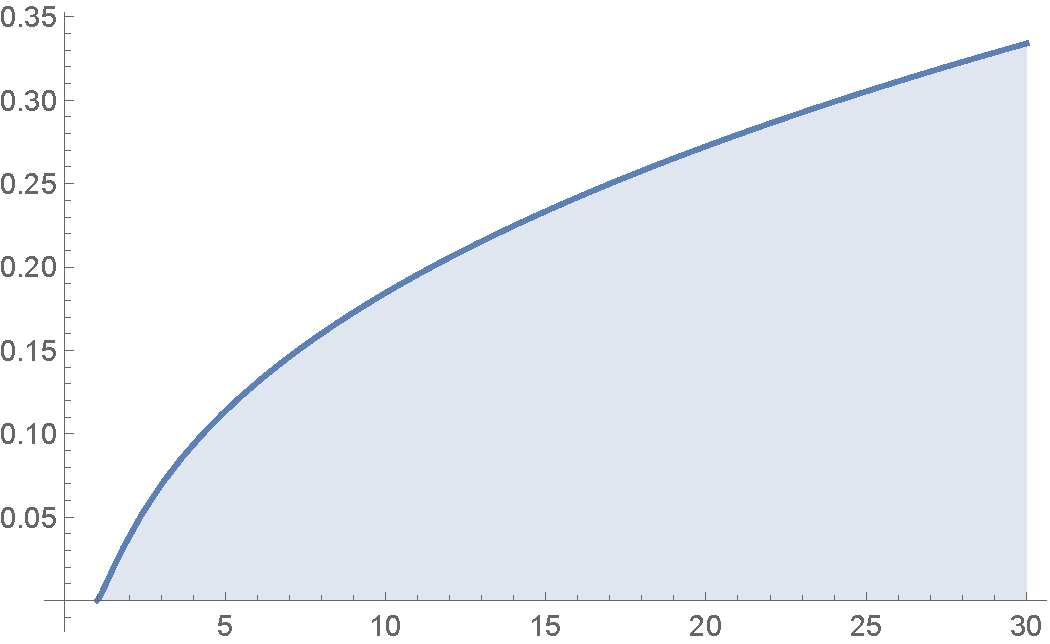
\includegraphics[width=1\textwidth]{Figures/Discriminant_dependence.pdf}
\end{figure}\label{discriminant}
In \autoref{discriminant}, the shaded area represent the conditions for the system to have damped oscillation.
\clearpage
\section{Time for intentional infection to gain advantage over non-intentional infection}
My old ``Time to advantage'' plot is the following.
\begin{figure}[H]
  \caption{Time for intentional infection to gain advantage over non-intentional infection}
  \centering
  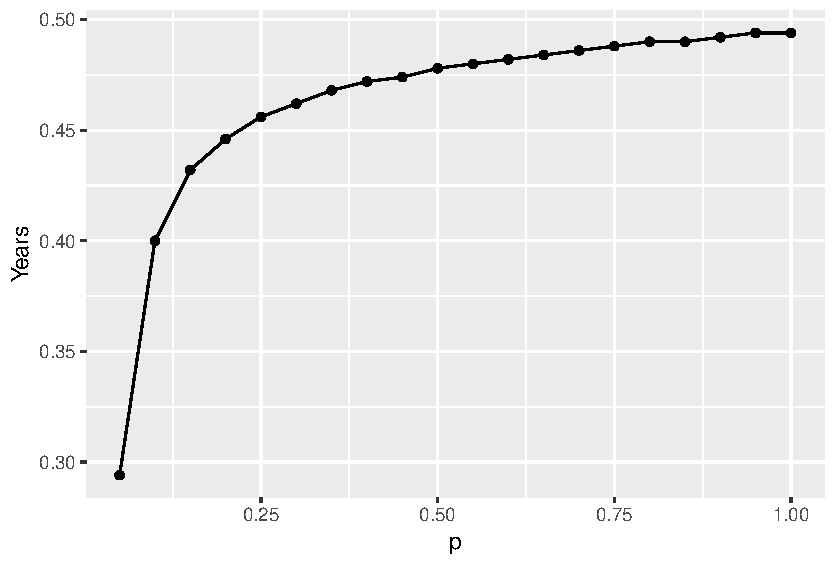
\includegraphics[width=1\textwidth]{Figures/Time_to_advantage_plot.pdf}
\end{figure}\label{advantage1}
Here it shows, with a lower proportion of intentional infection, we gain advantage relatively faster. This conclusion is misleading, because it is suggesting that, with a minimal proportion of intentional infection, we can minimize the time it takes to gain advantage.

We agreed that, if $p$ is small, though it gains advantage faster, it actually stays very close to non-intentional infection. In another word, the advantage is very insignificant.

Therefore, you suggested that, we can define ``Have advantage'' to be: mortality by intentional infection is at least 10\% lower than mortality with no intentional infection.
\begin{figure}[H]
  \caption{Time for mortality of intentional infection is at least 10\% lower than non-intentional infection}
  \centering
  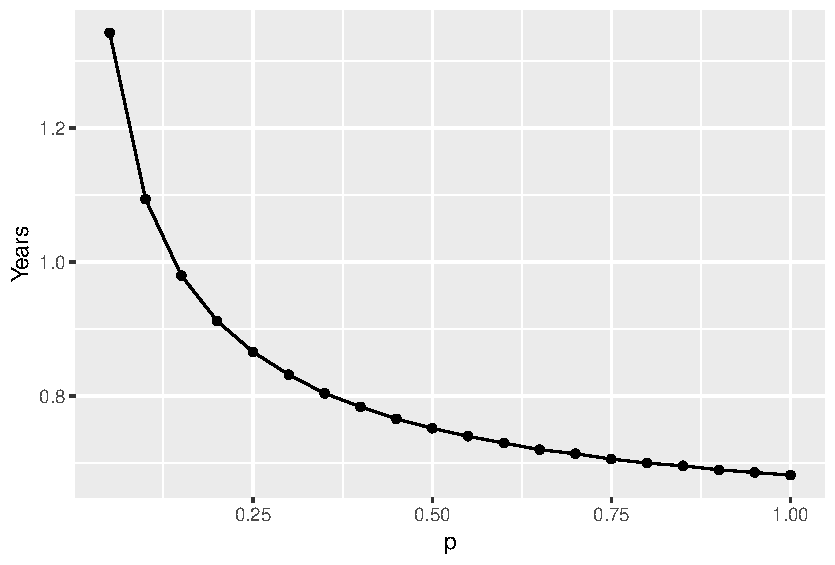
\includegraphics[width=1\textwidth]{Figures/New_time_to_advantage_plot.pdf}
\end{figure}\label{advantage2}
\autoref{advantage2} suggests, under our new definition of ``Have advantage'', a larger proportion $p$ is better.
\end{document}
